\documentclass[11pt]{article}

\usepackage[margin=1in]{geometry}
\usepackage{amsmath, amsthm, amssymb}
\usepackage{graphicx}
\usepackage{authblk}
\usepackage{apacite}
\usepackage{color}
\usepackage{setspace}

\newcommand{\TODO}[1]{\textcolor{red}{[TODO: #1]}}

\doublespacing{}

\title{Making decisions from samples with variable time costs}
\author{Jessica B. Hamrick (\texttt{jhamrick@berkeley.edu})}
\date{}\bibliographystyle{apacite}

\begin{document}

\maketitle

\section{Introduction}

% How do sample-based agents make decisions based on samples that take a variable amount of time?

% Evidence for sample (simulation based agents)

% Previous models have mostly compared people to an agent that takes an infinite number of samples.

% One and done: the best thing to do is take very few samples

% But one and done assumes that sampling cost is fixed -- what if samples take a variable amount of time?

\section{Sampling with variable time costs}

\citeA{Vul:2014ba} previously found that optimal sample-based agents should take only a few samples before making a decision, subject to the time cost of taking those samples. In this section, we first briefly summarize their formulation of the problem. Then, we describe how this formulation must be adjusted to account for samples with variable time costs.

\subsection{Background}

% briefly go over one and done math
Here, we consider the binary (or two-alternative forced choice) case, where an agent must choose one of two hypotheses, $H_0$ or $H_1$. The agent may take samples $X_i$ from a Bernoulli distribution parameterized by an unknown parameter $p$, and from these samples estimate $\hat{p}=\frac{1}{N}\sum_{i=1}^N X_i$, where $N$ is the total number of samples. Then, the decision rule which minimizes the probability of error is $\hat{H}(X_1,\ldots{},X_N)=H_0$ when $\hat{p}<0.5$ and $\hat{H}(X_1,\ldots{},X_N)=H_1$ when $\hat{p}>0.5$.

In the best possible case, the agent takes infinite samples and chooses the maximum \emph{a posteriori} (MAP) hypothesis with probability $p$. In practice, the agent cannot take infinite samples. Thus, to determine when to stop sampling (i.e., what the value of $N$ is), we use the \emph{sequential probability ratio test} \cite{wald1947sequential}. When using a SPRT strategy, the agent accumulates $Y_N=\sum_{i=1}^N 2X_i-1$, and stops either when $Y_N=T$ or $Y_N=-T$, for some threshold number of samples $T$. Independent of the number of samples actually taken, the probability of choosing $H_1$ given that $H_1$ is the MAP hypothesis is:
\begin{equation}
\Pr[\hat{H}(Y_N)=H_1\,|\,H_1]=\frac{p^T}{p^T+(1-p)^T},
\label{eq:pr-choose-h1}
\end{equation}
and so the marginal probability of correctly choosing the MAP hypothesis is:
\begin{equation}
\Pr[\mathrm{correct}]=\frac{p^{T+1}+(1-p)^{T+1}}{p^T+(1-p)^T}.
\label{eq:pr-correct}
\end{equation}
Then, the expected utility for a decision, given a threshold and the true probability, is:
\begin{equation}
\mathbb{E}[U\,|\,T,p]=\Pr[\mathrm{correct}]\cdot{}u^{(+)}+(1-\Pr[\mathrm{correct}])\cdot{}u^{(-)},
\label{eq:expected-utility}
\end{equation}
where $u^{(+)}$ is the utility for a correct answer and $u^{(-)}$ is the utility for an incorrect answer.

We are interested not just in how much utility is gained from a single decision, but how much utility is gained from \emph{each additional sample}. Under the SPRT strategy, the probability of taking $N$ samples and then choosing $H_1$ is:
\begin{equation}
\Pr[N,H_1\,|\,T,p]=\left(\frac{2^N}{2T}\right)p^{\frac{N+T}{2}}(1-p)^{\frac{N-T}{2}}\sum_{\nu=1}^{2T-1}\cos\left(\frac{\nu\pi}{2T}\right)^{N-1}\sin\left(\frac{\nu\pi}{2T}\right)\sin\left(\frac{\nu\pi}{2}\right)
\end{equation}
for $N\geq T$ and where $N$ is of the same parity as $T$ \cite[ch.~XIV, eq. 5.7]{Feller:1968ut}. Because we are dealing with binary hypotheses, the marginal probability of $N$ samples is then:
\begin{equation}
\Pr[N\,|\,T,p]=\Pr[N,H_1\,|\,T,p]+\Pr[N,H_1\,|\,T,1-p].
\label{eq:pr-n}
\end{equation}

\begin{figure}[t]
    \begin{center}
        \includegraphics[width=\textwidth]{figures/thresholds.pdf}
        \caption{\textbf{Rates of return and optimal thresholds.} In all plots, each line corresponds to a particular cost ratio, $t_a/t_s$. Black dots in the left two subplots show the optimal threshold $T^*$ and corresponding rate of return for each line. Left subplot: rates of return for a fixed time cost. Middle subplot: rates of return for a variable time cost. The distribution of $t_s$ was calculated empirically from simulations of a ball bouncing in a box (see Section \ref{sec:model}). Right subplot: difference in rates of return between the variable time cost and fixed time cost, approximated with Equation \ref{eq:ror-diff}.}
        \label{fig:rors}
    \end{center}
\end{figure}

Putting together Equations \ref{eq:expected-utility} and \ref{eq:pr-n}, the expected rate or return, or utility over time, is:
\begin{equation}
\mathbb{E}[U/t\,|\,T,t_a,t_s]=\int_0^1 \sum_{N=T}^\infty \frac{\mathbb{E}[U\,|\,T,p]\cdot{}t_a}{Nt_s+t_a}\Pr[N\,|\,T,p]\Pr[p]\ \mathrm{d}p,
\label{eq:ror-fixed}
\end{equation}
where $t_s$ is the time it takes to draw a single sample, and $t_a$ is the time it takes to make a decision or execute an action \cite{Vul:2014ba}. Finally, given this equation, we can compute the optimal threshold for an agent using the SPRT strategy:
\begin{equation}
T^*=\mathrm{arg}\max_T \mathbb{E}[U/t\,|\,T,t_a,t_s].
\label{eq:optimal-threshold}
\end{equation}

The rate of return and corresponding optimal thresholds for a variety of time costs, as computed by Equations \ref{eq:ror-fixed} and \ref{eq:optimal-threshold}, are shown in the left subplot of Figure \ref{fig:rors}.

\subsection{Variable time costs}

% convert one and done math to variable time costs
We now turn to the case where $t_s$ is variable and unknown. Let $t_N:=\sum_{i=1}^N t_s^{(i)}$ be the time it takes to draw $N$ samples. Then, the rate of return becomes:
\begin{equation}
\mathbb{E}[U/t\,|\,T,t_a]=\int_0^1 \sum_{N=T}^\infty \mathbb{E}[U\,|\,T,p]\cdot{}t_a\cdot{}\mathbb{E}\left[\frac{1}{t_N+t_a}\right]\Pr[N\,|\,T,p]\Pr[p]\ \mathrm{d}p.
\label{eq:ror}
\end{equation}

Because $t_N$ is always positive, $(t_N+t_a)^{-1}$ is convex. Using Jensen's inequality:
\begin{equation}
\mathbb{E}\left[\frac{1}{t_N+t_a}\right]\geq \frac{1}{N\cdot{}\mathbb{E}[t_s]+t_a},
\end{equation}
where the right hand side of the inequality corresponds to the original formulation by \citeA{Vul:2014ba}. Thus, the rate of return when the time cost is unknown will always be greater than when it is known. Intuitively, this makes sense: when an agent knows less to begin with, the samples it takes will give it more information, ultimately resulting in a higher rate of return.

We can approximate the extent to which samples are more useful when the time cost is unknown by computing using a Taylor expansion around $N\cdot{}\mathbb{E}[t_s]$:
\begin{equation}
\mathbb{E}\left[\frac{1}{t_N+t_a}\right]\approx \frac{1}{N\cdot{}\mathbb{E}[t_s]+t_a}+\frac{\mathrm{Var}(t_N)}{(N\cdot{}\mathbb{E}[t_s]+t_a)^3}-\ldots{}
\end{equation}
Thus, the difference is approximated by:
\begin{equation}
\mathbb{E}\left[\frac{1}{t_s+t_a}\right]-\frac{1}{N\cdot{}\mathbb{E}[t_s]+t_a}\approx \frac{\mathrm{Var}(t_N)}{(N\cdot{}\mathbb{E}[t_s]+t_a)^3}
\end{equation}
Plugging this back into Equation \ref{eq:ror}, we obtain the overall difference on the rate of return:
\begin{equation}
\mathbb{E}[U/t\,|\,T,t_a]=\int_0^1 \sum_{N=T}^\infty \mathbb{E}[U\,|\,T,p]\cdot{}t_a\cdot{}\frac{\mathrm{Var}(t_N)}{(N\cdot{}\mathbb{E}[t_s]+t_a)^3}\Pr[N\,|\,T,p]\Pr[p]\ \mathrm{d}p.
\label{eq:ror-diff}
\end{equation}

In practice, this difference is quite small. The middle subplot of Figure \ref{fig:rors} shows the rates of return using a variable time cost,\footnote{The times used for this plot were computed empirically using physical simulations of a ball boucing in a box. See Section \ref{sec:model} for details.} and the right subplot shows the difference computed from \ref{eq:ror-diff}. Even the largest difference, which occurs at $T=1$ and $t_a=\mathbb{E}[t_s]$, is so small that it does not change the value of $T^*$; the difference would need to be about 100 times greater in order to have an effect. Using different distributions for $\Pr[t_s]$ may have larger effects, but even these are not substantial. For example, using a uniform distribution can change $T^*$ from 0 to 1 for smaller cost ratios.

To summarize, we find that the introduction of uncertainty into the time cost has very little effect. The implication of this result is that even if it \emph{does} takes a variable amount of time to draw a sample, an agent need not bother taking its uncertainty into account: it can rely solely on its estimate of the average sample time to determine an optimal threshold.

\section{Case study: intuitive physics}

How well does the optimal SPRT strategy actually match up with human responses on a task with variable sample costs? To answer this question, we considered the scenario where participants watch a ball bouncing around in a box, and must determine whether the ball will go through a hole in the wall.

\subsection{Model}
\label{sec:model}

% describe model from sources of uncertainty
As discussed in the introduction, recent research suggests that people can reason about physical scenarios by running noisy physics simulations \cite<e.g.>{Smith2012,Battaglia2013,Smith:2013ug,Smith:2013th,Ullman:2014ut}. Here, we assume this to be the case, and use the model from \citeA{Smith2012}. Briefly, their model incorporates four sources of uncertainty into the physical simulations: perceptual uncertainty over the position of the ball ($\sigma_p$), uncertainty in the initial direction of velocity ($\kappa_v$), ongoing uncertainty in the direction of movement ($\kappa_m$), and uncertainty in the bounce angle ($\kappa_b$). To determine the probability that the ball goes in the hole, we simulated $M=10000$ samples from the model. For each sample, we computed whether the ball went in the hole, and then averaged over all the samples.

\subsection{Methods}

\subsubsection{Participants}

We recruited $N=328$ participants on Amazon's Mechanical Turk using the psiTurk \cite{McDonnell12} experimental framework. Participants were treated in accordance with UC Berkeley IRB standards and were paid \$0.60 for approximately 6.5 minutes of work. Participants were randomly assigned to one of eight conditions, which determined which stimuli they judged based on a latin-square design (see Stimuli). Additionally, we excluded $N=8$ participants from analysis for answering incorrectly on more than one control trial (see Stimuli), leaving a total of $N=320$ participants.

\subsubsection{Stimuli}

% include figure of stimulus
The stimuli consisted of animations depicting a blue ball with a radius of 10px bouncing around in a box with dimensions 900px $\times$ 650px. All stimuli consisted of two separate animations. The first was he stimulus presentation, which had a duration of 0.775 seconds and depicted the ball moving in a particular direction. The second animation was the feedback, which picked up immediately where the first animation left off, and which had a duration of 1.5 seconds and depicted the ball either going into the hole or bouncing off the wall that contained the hole.\footnote{To enforce the constraint that the ball always travel the same distance during the feedback animation, the $x$-coordinate of the wall with the hole in it was allowed to vary across stimuli.} During the feedback animation, the ball could bounce on the other walls either 0, 1, or 2 times before going into the hole hitting the wall with the hole in it. In both animations, the ball had a velocity of 400px/s. Additionally, in the animations, the path that the ball had traveled so far was drawn with a faded gray line (see Figure \ref{fig:experiment}).

There were 48 different initial animations, and for each of these intial animations, there were four different types of feedback and two different hole sizes, giving a total of eight versions of each stimulus. The four feedback types were: ``straight hit'', where the ball went directly through the center of the hole; ``far miss'', where the ball missed the hole by a wide margin; ``close hit'', where the ball just barely went through the hole; and ``near miss'', where the ball just barely missed the hole. The two hole sizes were 100px and 200px.

In order to ensure that participants never saw the same initial animation twice, we used a latin-square design of Initial Animation $\times$ Hole Type $\times$ Hole Size. Thus, each participant saw each initial animation exactly once, each hole type exactly 12 times, and each hole size exactly 24 times.

In addition to the 48 experimental trials, there were seven instruction trials and eight control trials, which were the same for all participants. The control trials were designed to be extremely easy and were either of type ``straight hit'' (with a hole size of either 300px or 350px) or ``far miss'' (with a hole size of 100px). Thus, participants saw a total of 63 trials throughout the experiment.

\begin{figure}[t]
    \begin{center}
        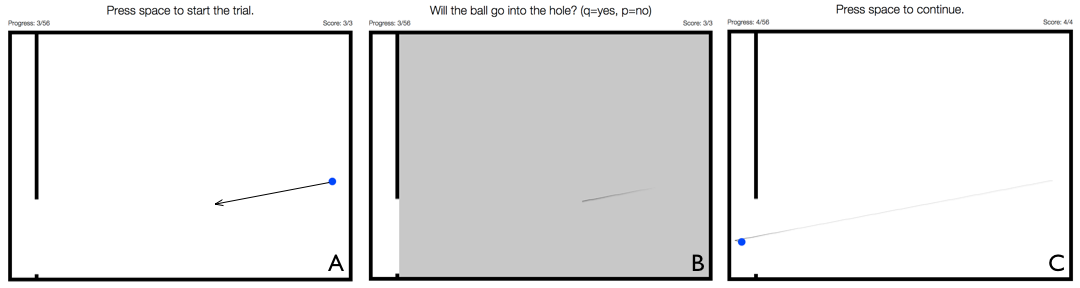
\includegraphics[width=\textwidth]{figures/experiment.png}
        \caption{\textbf{Example experimental trial.} Each panel shows a different part of the trial. The left panel shows the initial screen presented to the participant. The middle panel shows the occluded ball, after observing the stimulus presentation. The faded gray line shows the path the ball took during the initial presentation. The right panel shows the final position of the ball, after observing the feedback. As in the middle panel, the faded gray line shows the path of the ball.}
        \label{fig:experiment}
    \end{center}
\end{figure}

\subsubsection{Procedure}

The experiment was divided into two phases: the training phase, and the experimental phase. During the training phase, participants made judgments on the seven instruction trials in order to get used to the task. During the experimental phase, participants made judgements on the 48 experimental trials, presented in a random order, as well as the eight control trials, which were also shown in a random order, but interspersed with the experimental trials such that every 8th trial was a control trial.

On each trial, participants were shown the scene, including the initial position of the ball and the location of the hole. Participants were instructed to press the ``space'' key to begin the trial. Immediately upon pressing ``space'', the initial stimulus presentation began. As soon as the initial stimulus animation concluded, a gray box was drawn over the screen, occluding the ball (but not the line depicting the path it had traveled so far; this was left in as a reminder to participants of where the ball had come from). Participants were asked, ``will the ball go in the hole?'', and were instructed to press `q' to respond in the affirmative, and `p' to respond in the negative. Immediately after responding, text appeared saying ``Correct!'' or ``Incorrect.'', depending on the participants' response. Additionally, the gray occluder was removed, and participants were shown the feedback animation. After the feedback animation was complete, the final frame of the animation remained on the screen until participants pressed ``space'' to advance to the next trial. Figure \ref{fig:experiment} shows a few frames from one of the experimental trials.

\subsection{Results}

\begin{figure}[h]
    \begin{center}
        \includegraphics[width=0.5\textwidth]{figures/human-pct-vs-rt.pdf}
        \caption{\textbf{Response times as a function of response.}}
        \label{fig:pct-vs-rt}
    \end{center}
\end{figure}



\section{Discussion}

\bibliography{references}

\end{document}
